\subsection{Onda completa con derivación central}
El circuito con filtro de $470[\mu\text{F}]$ pueden verse en la
\textbf{figura~\ref{circuito06}} para el rectificador de onda completa con
derivación central.

\begin{figure}[!h]
\centering
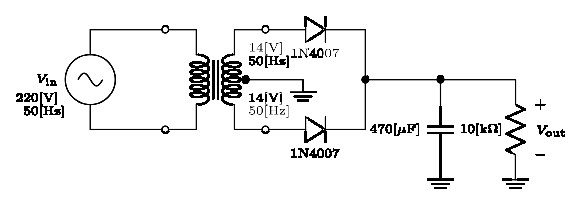
\includegraphics[scale=1.1]{diagramas/06.derivacion_central2.eps}
\caption{Rectificador de onda completa con transformador de \\
derivación central y filtro.}
\label{circuito06}
\end{figure}

\subsubsection{Simulación}
Se utilizó el software \emph{Quite Universal Circuit Simulator.} versión 23.3.1
para la simulación del rectificador de onda completa con transformador de
derivación central con filtro, este puede verse en la
\textbf{figura~\ref{simulacion06}}.

\begin{figure}[!h]
\centering
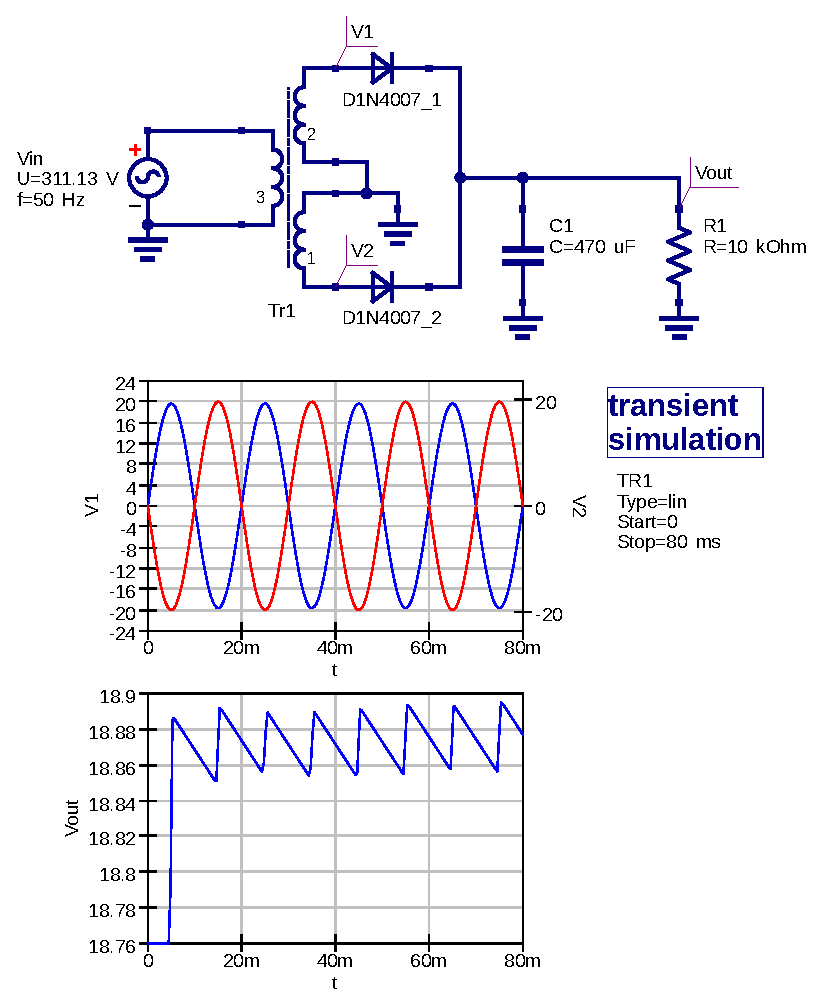
\includegraphics[scale=0.75]{simulacion/06.derivacion_central2.eps}
\caption{Simulación del rectificador de onda completa con \\
derivación central y filtro.}
\label{simulacion06}
\end{figure}

\subsubsection{Laboratorio}
Se presenta el rectificador de onda completa con el transformador de derivación
central y filtro armado en laboratorio y su medición de voltaje de salida en la
carga, en la \textbf{figura~\ref{laboratorio08}}.

\begin{figure}[!h]
\centering
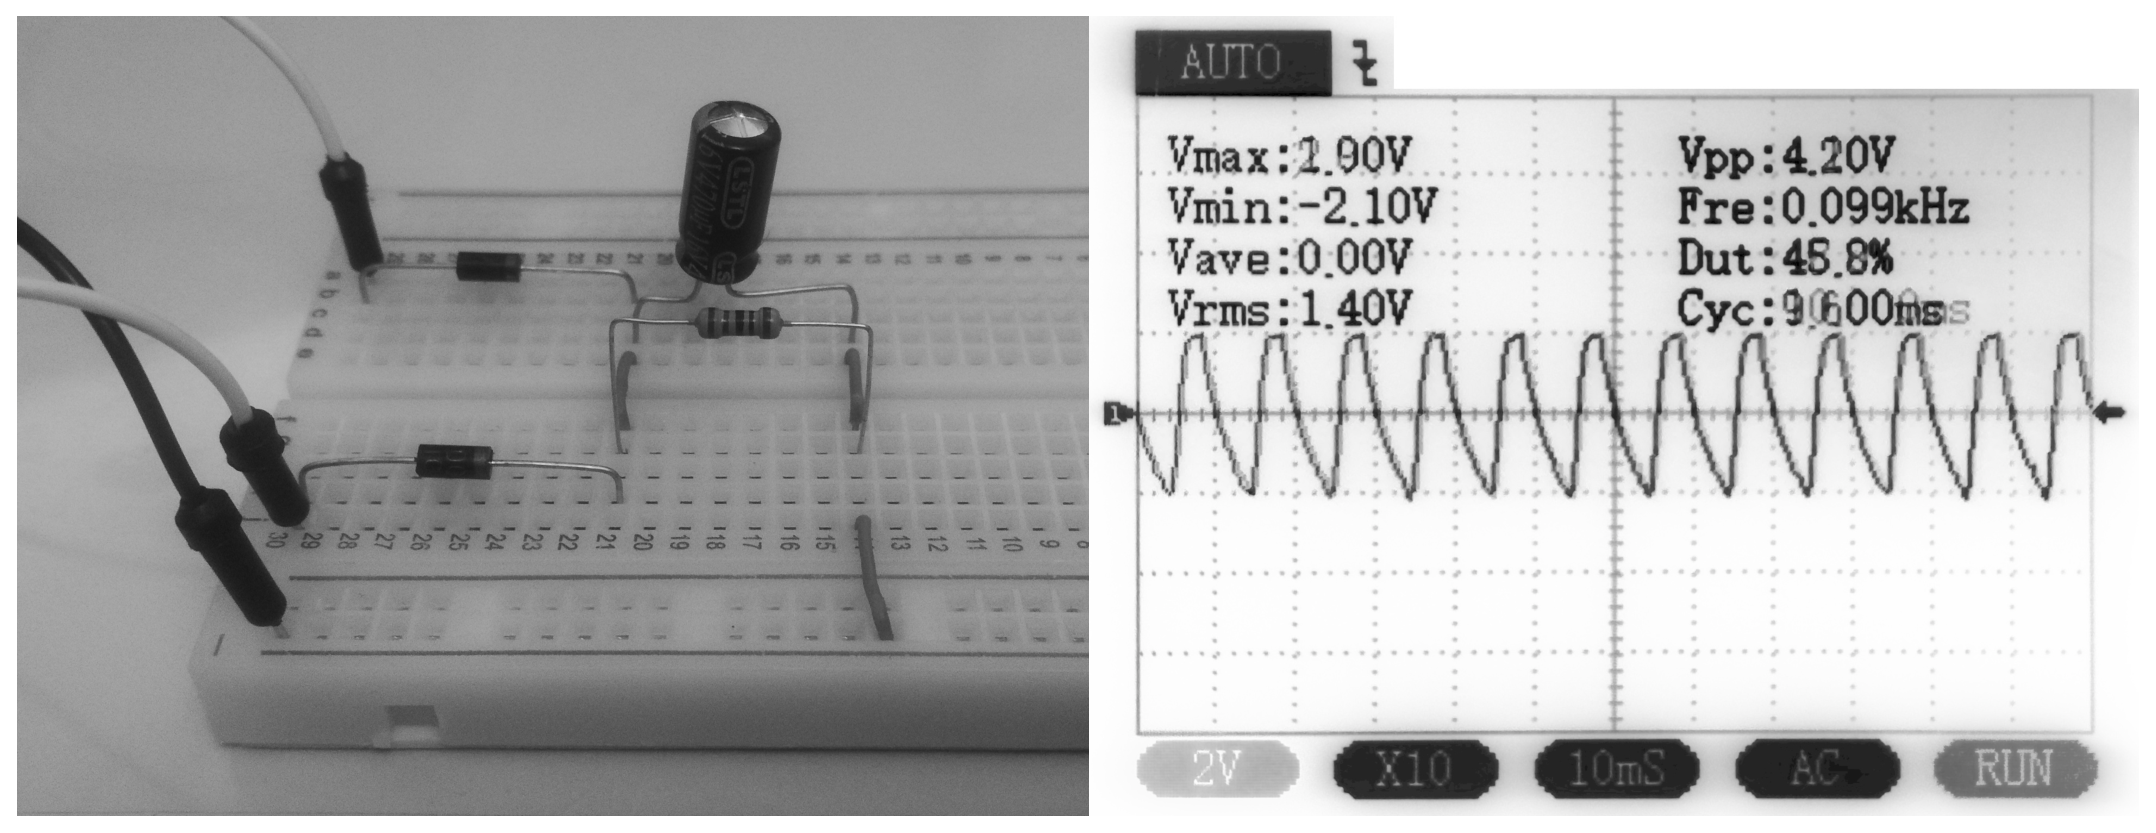
\includegraphics[scale=0.34]{fotos/06.derivacion_central2.eps}
\caption{Rectificador de onda completa con derivación central y filtro.}
\label{laboratorio08}
\end{figure}

